\chapter{Future Work}

This project provides an initial profile-aware auditing framework for measuring differential dark pattern exposure in mobile applications. However, as discussed in the limitations, the current framework remains partly manual, uses static profiles, and evaluates a bounded set of applications and interaction steps. Future work can extend the framework in several directions so that profile-conditioned dark pattern exposure can be measured more automatically, more realistically, and at a larger scale.

\section{Automatic DPS Detection}

A major direction for future work is the automatic detection of DPS dimensions from mobile interface screenshots and interaction traces. In the current project, DPS annotation relies on human judgment, which is useful for interpretability but costly to scale. Manual annotation also introduces potential inconsistency, especially when a screenshot contains ambiguous interface elements or multiple dark pattern mechanisms at the same time. Future versions of the framework could therefore combine optical character recognition, computer vision, UI element detection, and multimodal large language models to identify dark pattern evidence automatically.

For example, OCR could extract textual cues such as countdown messages, urgency phrases, discount claims, membership reminders, or refusal-related wording. Computer vision models could identify layout-level features such as button size asymmetry, color salience, hidden close buttons, pop-up overlays, and obstructed exit paths. UI element detection could further help distinguish between accept buttons, reject buttons, checkout links, recommendation cards, and subscription prompts. These signals could then be mapped into the seven DPS dimensions: Interface Interference, Friction, Pressure, Contextual Deception, Sneaking, Nagging, and Forced Action. Recent work on dark pattern taxonomy and detection suggests that automated classifiers may help reduce the burden of manual inspection, although full automation should still be treated carefully because dark pattern interpretation often depends on context \cite{li2024comprehensive,mathur2019darkpatterns}.

A practical future system could use a hybrid pipeline. First, screenshots and UI trees would be processed by OCR and visual detectors. Second, a dark pattern classifier or multimodal model would produce candidate DPS labels with confidence scores. Third, human annotators would only review uncertain or high-risk cases. This would reduce annotation cost while preserving quality control. Such an approach would make it possible to audit many more applications and interaction records than the current 1,440-record experiment.

\section{LLM Agent-based App Exploration}

Another important extension is to replace simple probabilistic action generation with LLM agent-based mobile app exploration. In the current framework, user behavior is modeled as a profile-conditioned probability distribution over actions. This design is controlled and reproducible, but it simplifies how real users interact with mobile applications. Real users do not merely sample actions from fixed probabilities; they read interface content, react to recommendations, compare options, abandon tasks, and enter decision-related flows based on evolving goals.

Future work could use LLM agents to explore apps in a more natural and goal-directed manner. Each agent could be assigned a profile-specific objective, such as searching for high-value electronics, browsing casually without purchase intent, or finding coupons and limited-time discounts. The agent could observe the current screen, interpret interface content, decide the next action, and record why that action was chosen. This would allow the audit to capture more realistic trajectories than fixed action templates alone.

LLM agents could also enter decision-related flows more intelligently. For instance, a high-payment shopping agent might compare recommended items and proceed toward checkout when the interface appears relevant, while a bargain-hunter agent might actively search for discount codes, flash sales, or membership rewards. This would make the framework closer to real profile-conditioned behavior while still preserving audit control. Similar to sock-puppet and agent-based audits in recommendation systems, the key challenge would be balancing realism with reproducibility \cite{srba2023youtube,haroon2023youtubeaudit}. Future work should therefore log agent prompts, observations, actions, and decision rationales so that the exploration process remains inspectable.

\section{Dynamic User Modeling}

The current framework uses static user profiles. Each profile has a predefined interest distribution and behavior distribution, and these settings remain unchanged during the 30-step interaction process. This is useful for a first controlled experiment, but it does not fully represent real users. In actual mobile applications, user profiles may evolve as users search, click, browse, ignore recommendations, open payment pages, or repeatedly respond to pop-ups.

Future work could model user profiles dynamically. Instead of treating profile \(A_t\) as fixed, the framework could update the profile after each interaction according to the user’s history:

\[
A_{t+1} = f(A_t, history_t)
\]

In this formulation, \(A_t\) denotes the user profile at step \(t\), while \(history_t\) represents the accumulated interaction history up to that point. The function \(f\) updates the user representation based on observed actions, searched keywords, clicked items, dwell time, and decision-related visits. This would better reflect real users whose interests and behaviors are not static but change through interaction.

Dynamic user modeling would also allow the audit to examine whether dark pattern exposure increases, decreases, or changes type as a profile becomes more established. For example, a bargain-hunter profile might initially receive general shopping recommendations but gradually encounter more discount-related pressure or membership prompts. A high-payment profile might be routed more often into checkout-adjacent flows after repeated high-value searches. These possibilities should not be interpreted as causal claims without stronger evidence, but dynamic modeling would make such temporal patterns observable and testable. Prior work on user profiling and sequential recommendation provides useful conceptual support for this direction \cite{purificato2024usermodeling,lian2021multiinterest,hou2022unisrec}.

\section{Larger-scale Auditing}

The current experiment covers 16 applications, 3 profiles, and 30 steps per profile-app pair, producing 1,440 interaction records and 10,080 DPS labels. This scale is sufficient for a course project and demonstrates the feasibility of profile-conditioned exposure estimation. However, larger-scale auditing is necessary before making broader claims about mobile app ecosystems.

Future work could expand the framework across more applications, more categories, more geographic regions, more app versions, and longer observation windows. Different app categories may exhibit different dark pattern mechanisms. For example, food-delivery apps may show consistently high forced-action exposure, while shopping apps may show stronger pressure or interface interference around promotional and checkout flows. A larger audit could test whether these category-level patterns remain stable across platforms and regions.

Repeated audits over time would also be valuable. Mobile applications frequently update their interfaces, recommendation strategies, promotion mechanisms, and consent flows. A single audit captures only one time window. By repeating the same profile-conditioned audit monthly or across major app versions, researchers could observe whether dark pattern exposure is persistent, seasonal, or associated with specific platform updates. This would improve the generalizability and temporal validity of the framework.

\begin{figure}[htbp]
    \centering
    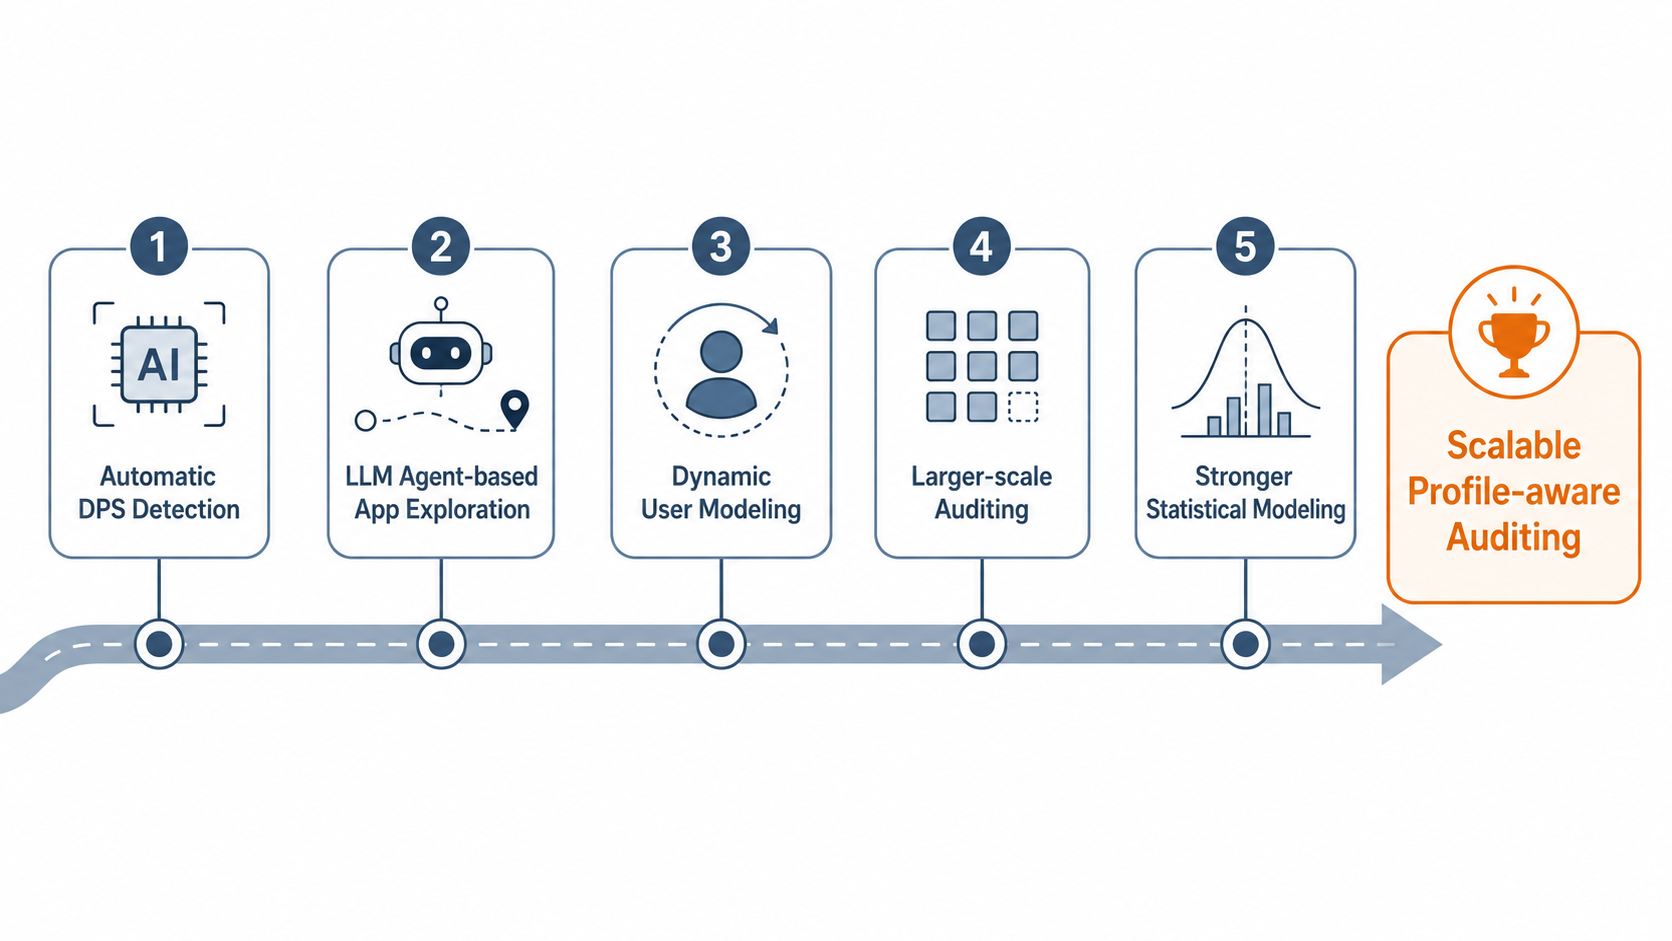
\includegraphics[width=0.95\linewidth]{figures/pictures/future_work_roadmap.png}
    \caption{Future Work Roadmap}
    \label{fig:future_work_roadmap}
\end{figure}

\section{Stronger Statistical Modeling}

Finally, future work can strengthen the statistical analysis of profile-dependent exposure. The current framework already uses profile-conditioned exposure estimation \(E(D \mid A)\), pairwise exposure differences \(\Delta(A_i, A_j)\), permutation tests, q-values, L1 distance, and Cramér’s V. These methods provide useful evidence of association between user profile and DPS exposure, but more advanced models could provide a clearer decomposition of where the differences come from.

Mixed-effects models could account for the fact that observations are nested within apps, app categories, profiles, and interaction steps. Bootstrap confidence intervals could quantify uncertainty around exposure estimates without relying too heavily on parametric assumptions. Longitudinal analysis could examine whether exposure converges, accumulates, or changes across interaction trajectories. These methods would make the framework more statistically robust, especially when extended to larger datasets.

A particularly important direction is causal mediation analysis or profile-action-DPS decomposition. In the current setting, a profile may receive different exposure partly because the platform personalizes the interface directly, but also partly because different profiles take different actions. For example, the high-payment profile may encounter more pressure-related exposure because it enters checkout pages more often, not necessarily because the platform directly targets that profile with pressure. Mediation analysis could help separate these possibilities by estimating how much of the profile difference is associated with action pathways such as search behavior, recommendation clicks, or decision-interface visits. Such analysis would not automatically prove causality, but it would provide a more careful way to distinguish direct profile-associated exposure from exposure mediated by interaction behavior.

Together, these future directions would extend the current framework from a controlled course-scale audit into a more automated, adaptive, and statistically rigorous system for studying personalized dark pattern exposure in mobile applications.
